%\newpage

\section{Inertial Range}\label{appInertial}


\textbf{\noindent
    In this section, we aim to verify that there is a reasonable range of scales, in terms of $\ell$, within which the simulations are not dominated by numerical diffusion, but rather by correctly simulated as they resolve the inertial range of the turbulent cascades.
    Therefore, we offer more examples that show VSFs of all three clouds at different times and considering different analysis approaches.
    In particular, we focus on the standard analysis (Sects.~\ref{results:normal} and~\ref{discussion:normal}, Figs.~\ref{pic:appInertial:examples_with_threshold_s_vs_l} and~\ref{pic:appInertial:examples_with_threshold_sl_vs_l}), the density threshold-less scenario (Sects.~\ref{results:densthres} and~\ref{discussion:densthres}, Figs.~\ref{pic:appInertial:examples_without_threshold_s_vs_l} and~\ref{pic:appInertial:examples_without_threshold_sl_vs_l}), and the impact analysis of different Jeans refinement levels (Sects.~\ref{results:refinement} and~\ref{discussion:refinement}, Figs.~\ref{pic:appInertial:examples_jeans_s_vs_l} and~\ref{pic:appInertial:examples_jeans_sl_vs_l}).
}
 	
\begin{figure*}
    \centering
    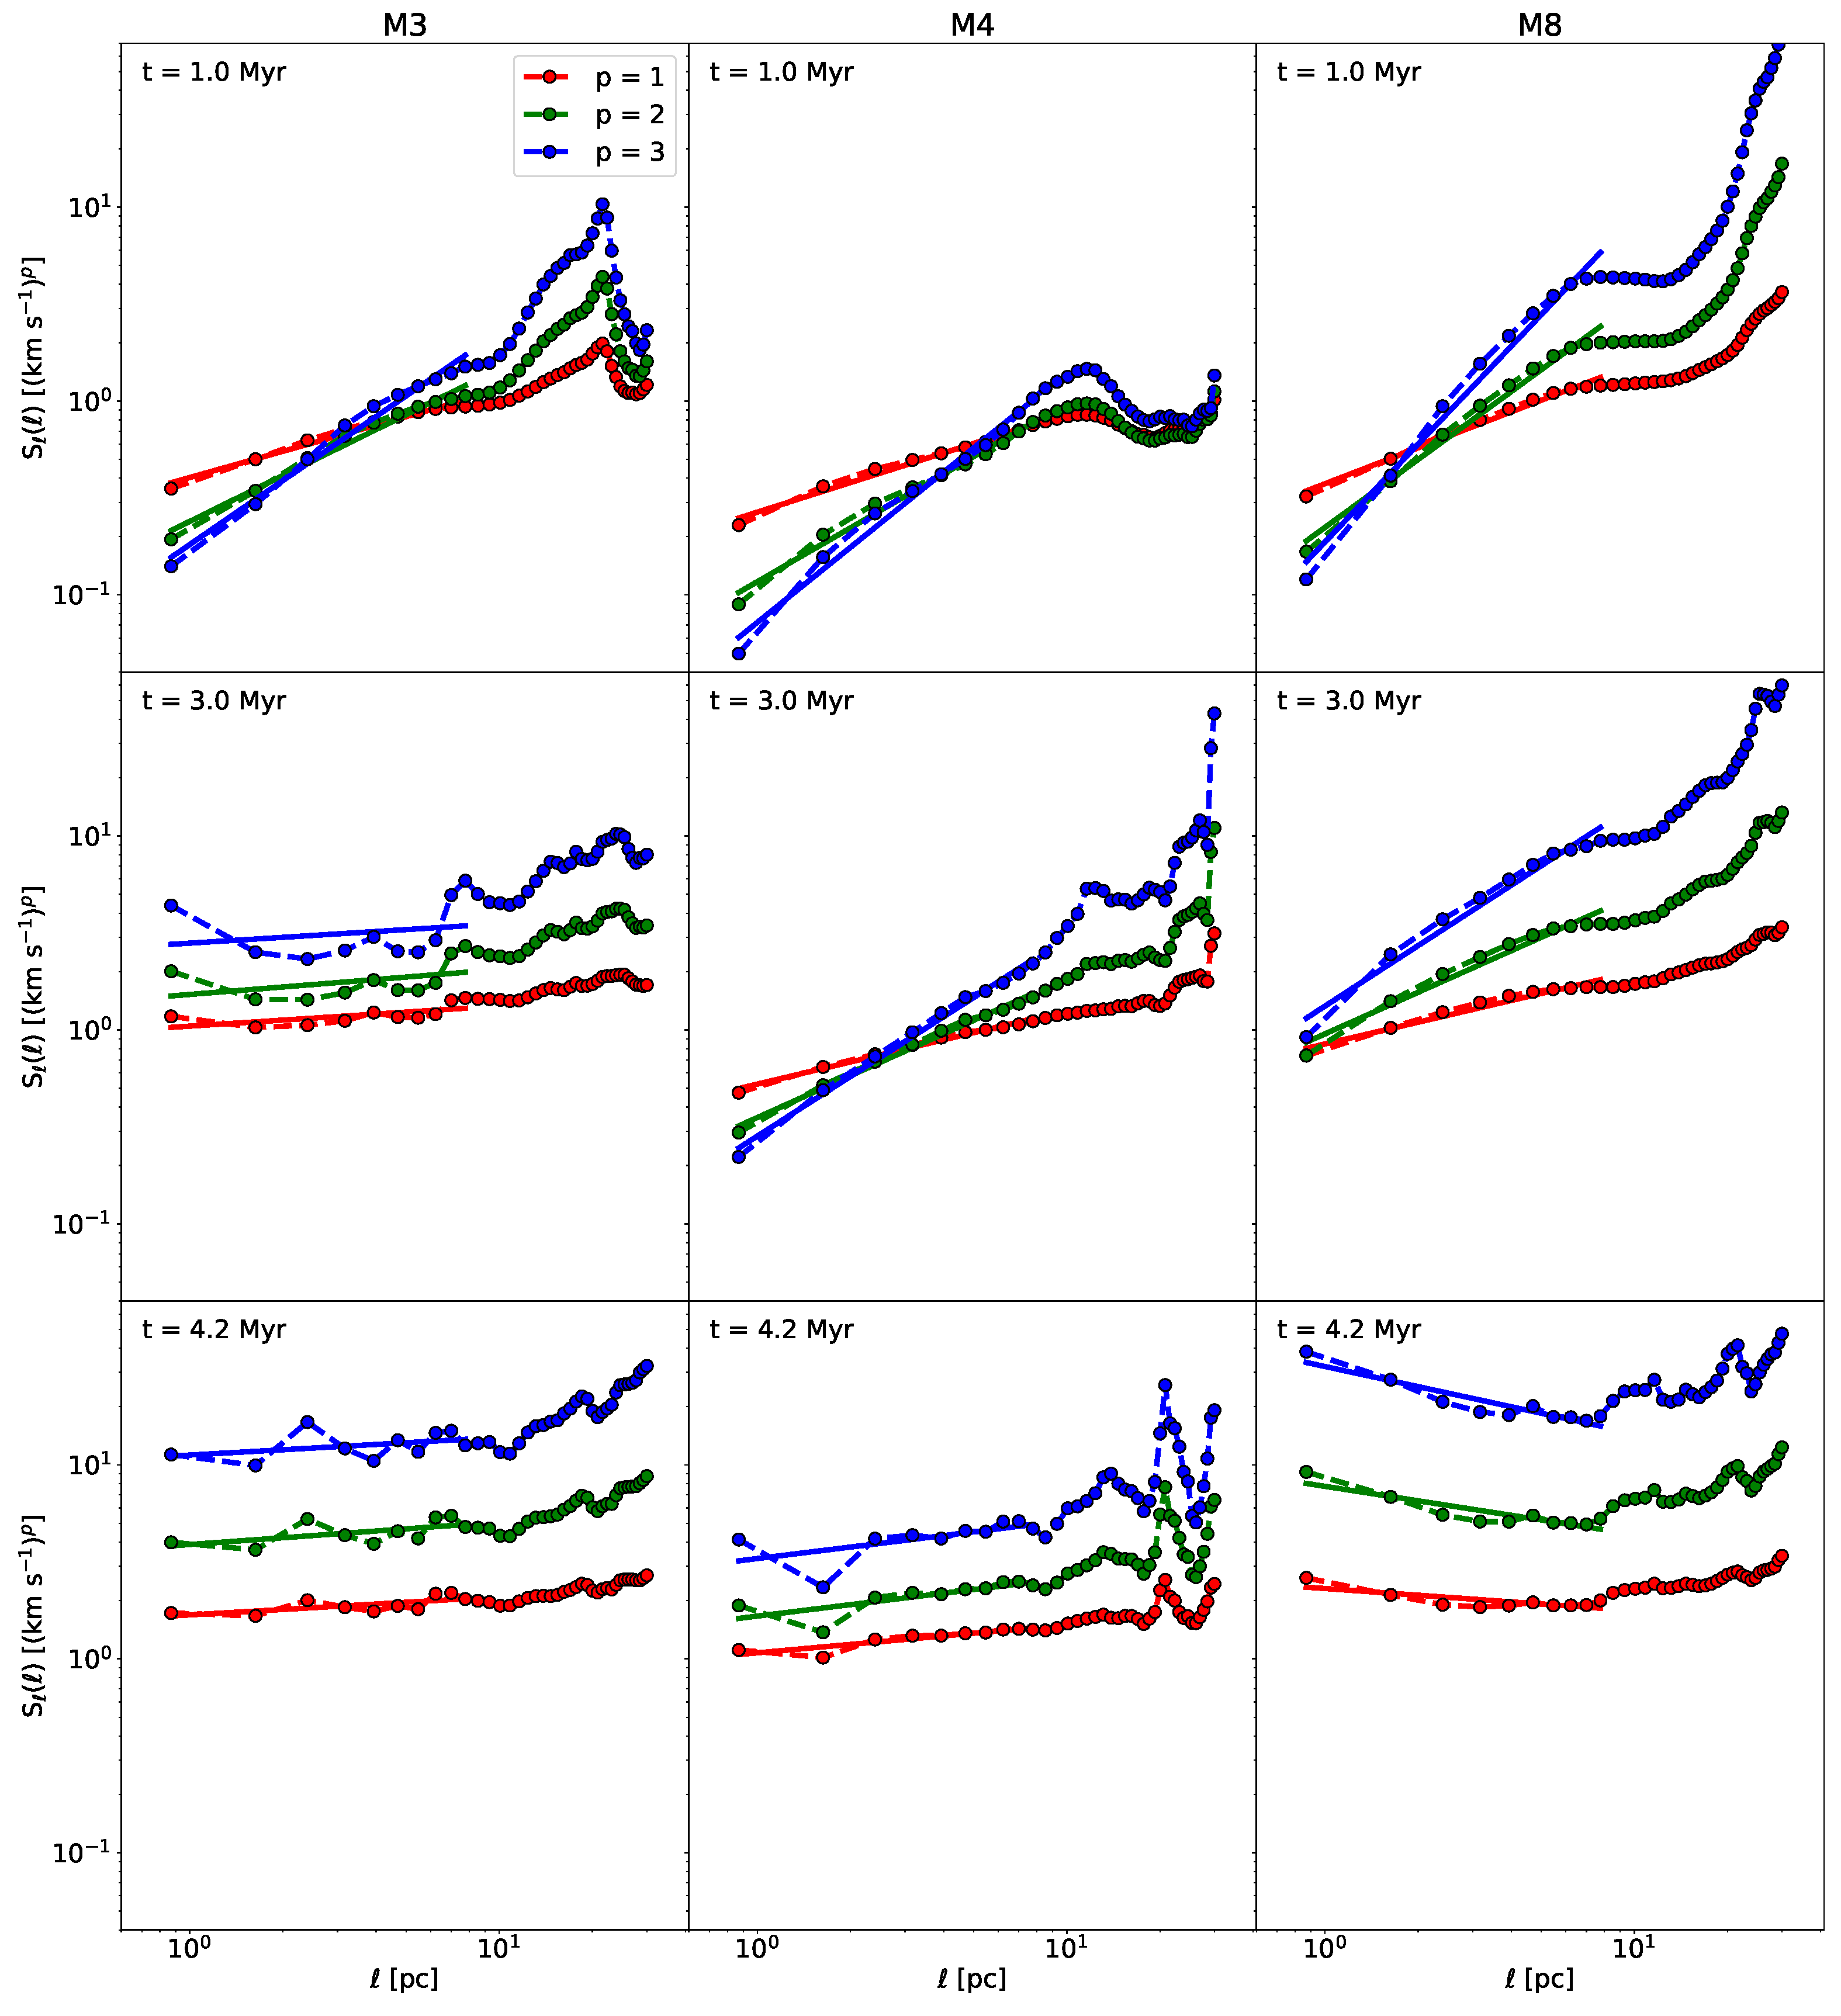
\includegraphics[width=\textwidth]{app_examples_wthres_s_l.pdf}
    \caption{
        The figures show additional examples of VSFs, based on data with density threshold, of (\textit{left} to \textit{right}) \texttt{M3}, \texttt{M4}, and \texttt{M8} as function of lag scale $\ell$ and order $p$. 
        The examples are given for three different time steps, namely (\textit{top} to \textit{bottom}) t~=~1.0~Myr, 3.0~Myr, and 4.2~Myr.
        The dots (connected by dashed lines) show the values computed from the simulations. 
        The solid lines represent the power-law relation fitted to the respective structure functions.
    }
    \label{pic:appInertial:examples_with_threshold_s_vs_l}
\end{figure*}
 	
 	
\begin{figure*}
    \centering
    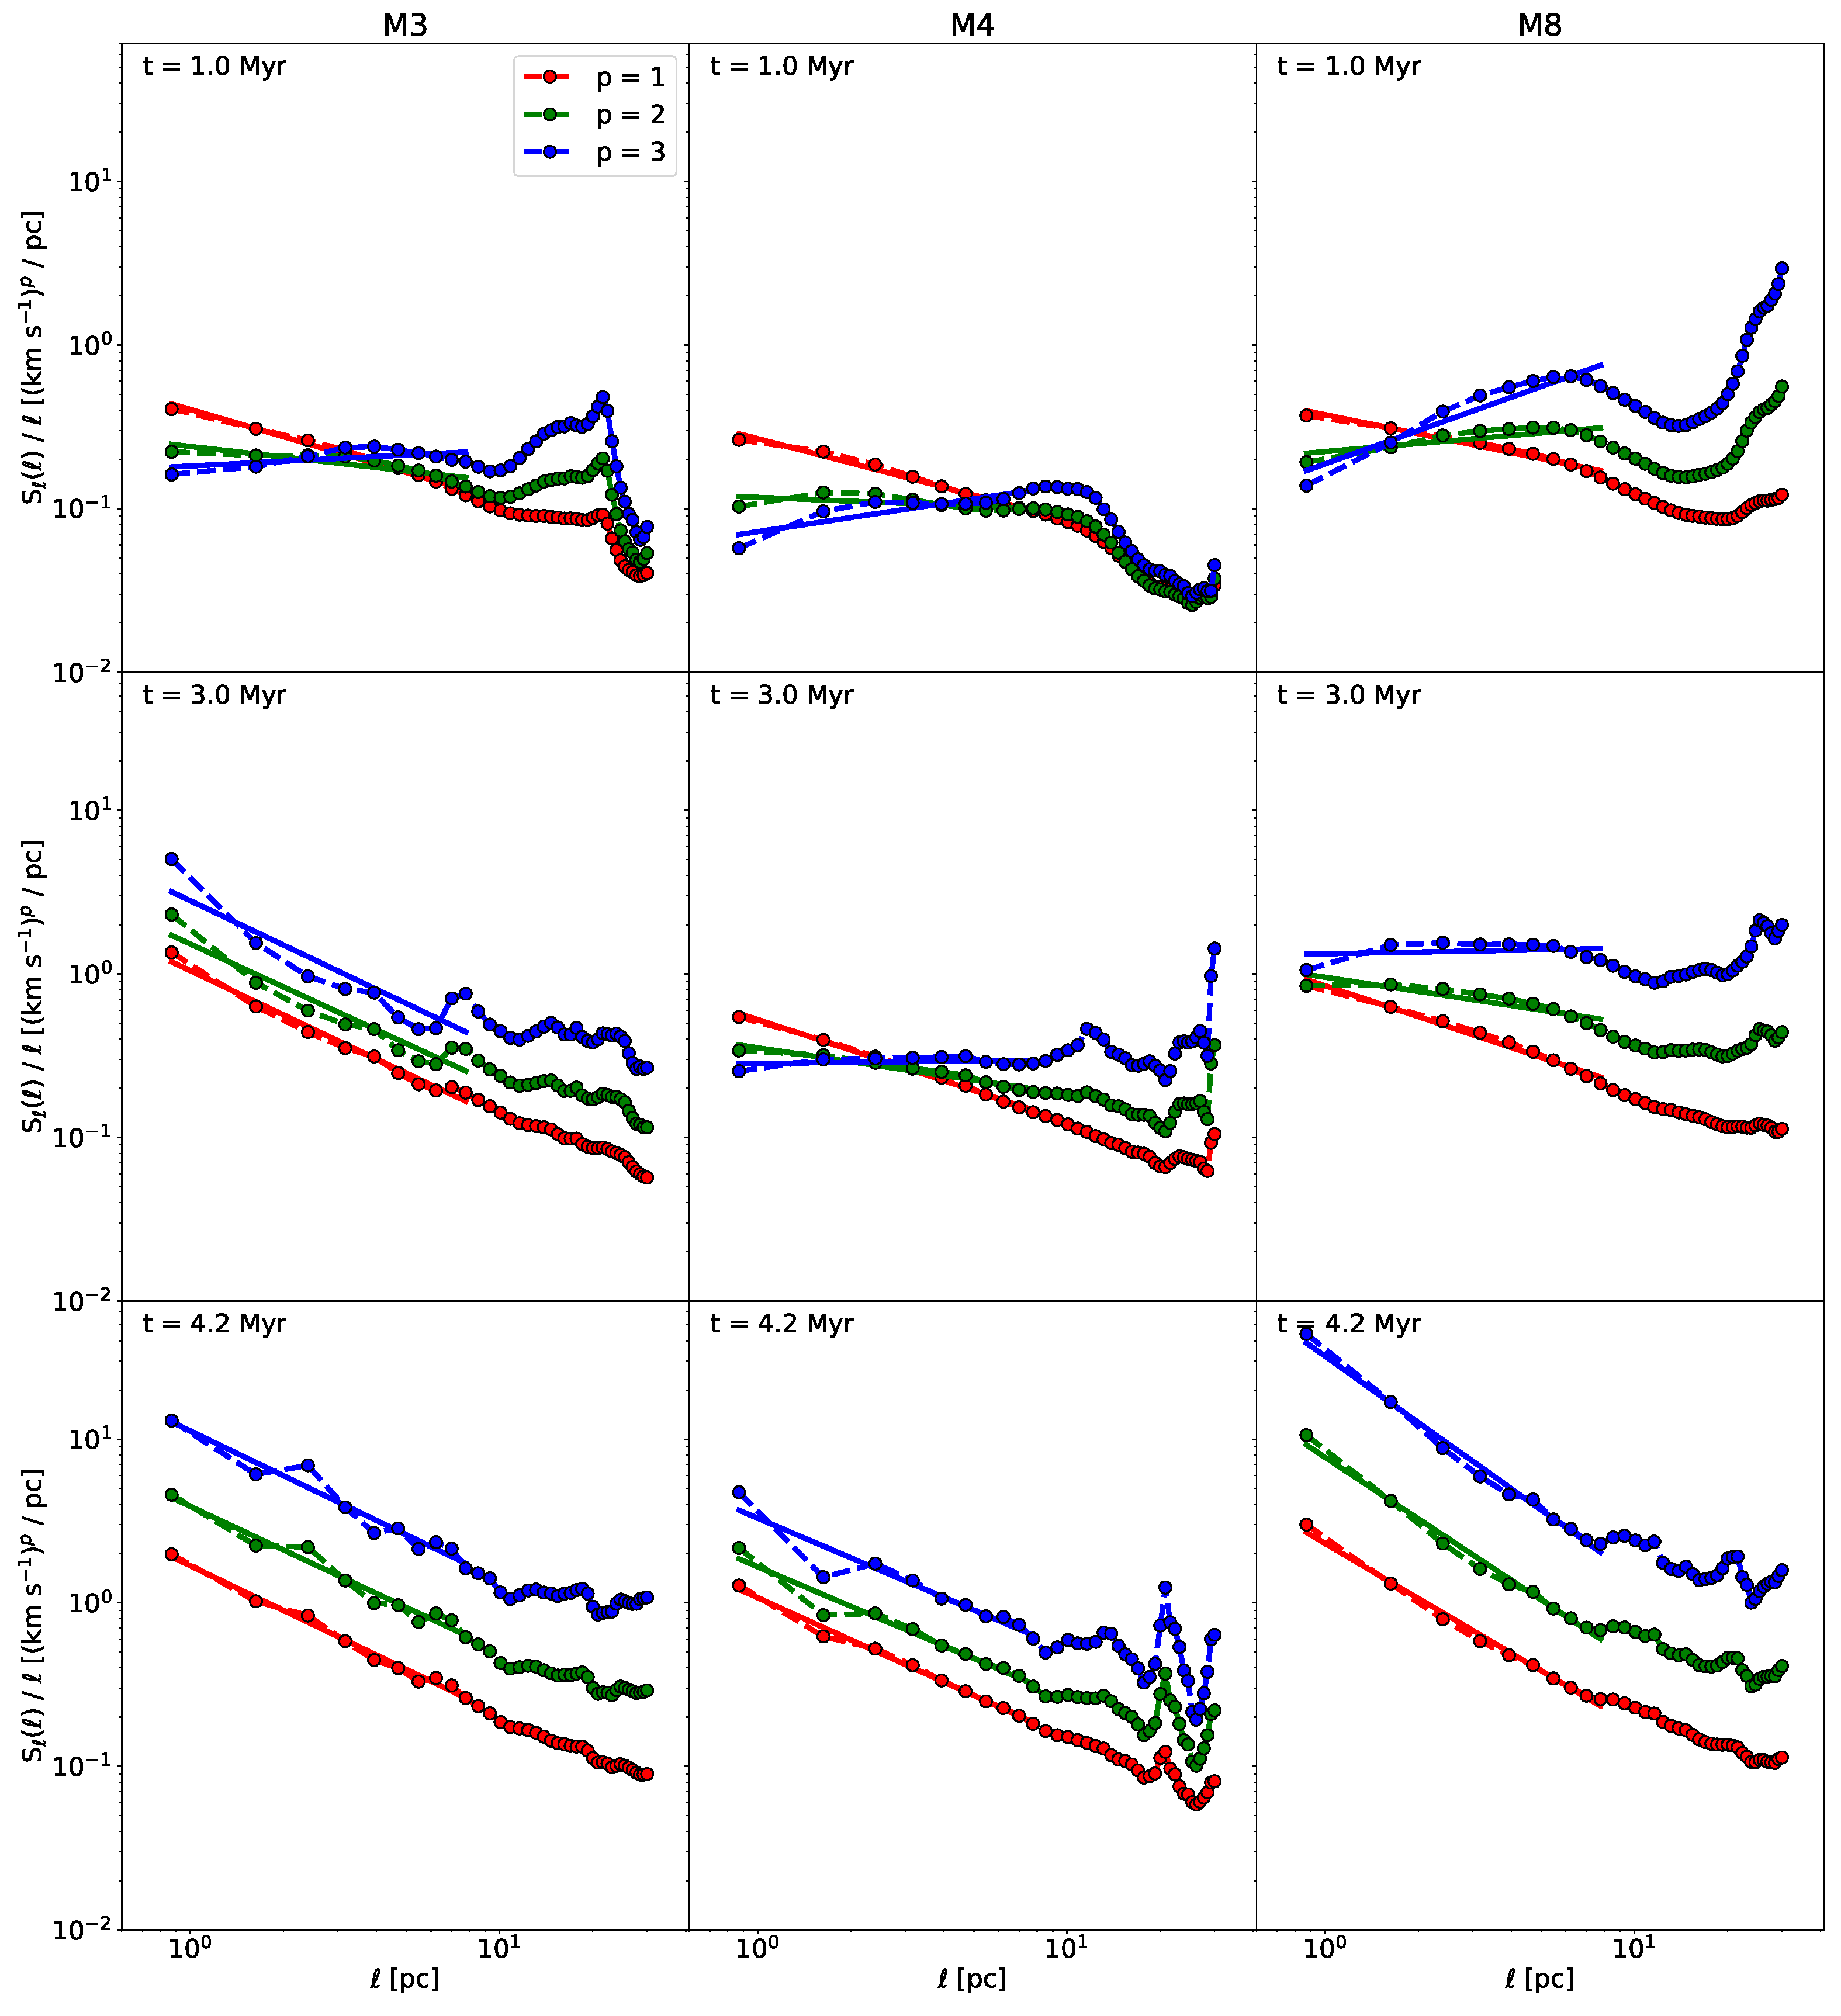
\includegraphics[width=\textwidth]{app_examples_wthres_sl_l.pdf}
    \caption{
        As Fig.~\ref{pic:appInertial:examples_with_threshold_s_vs_l}, but plotting the relation between S$_{\ell}$ / $\ell$ as function of lag scale $l$ and order $p$.
    }
    \label{pic:appInertial:examples_with_threshold_sl_vs_l}
\end{figure*}
 	
 	
\begin{figure*}
    \centering
    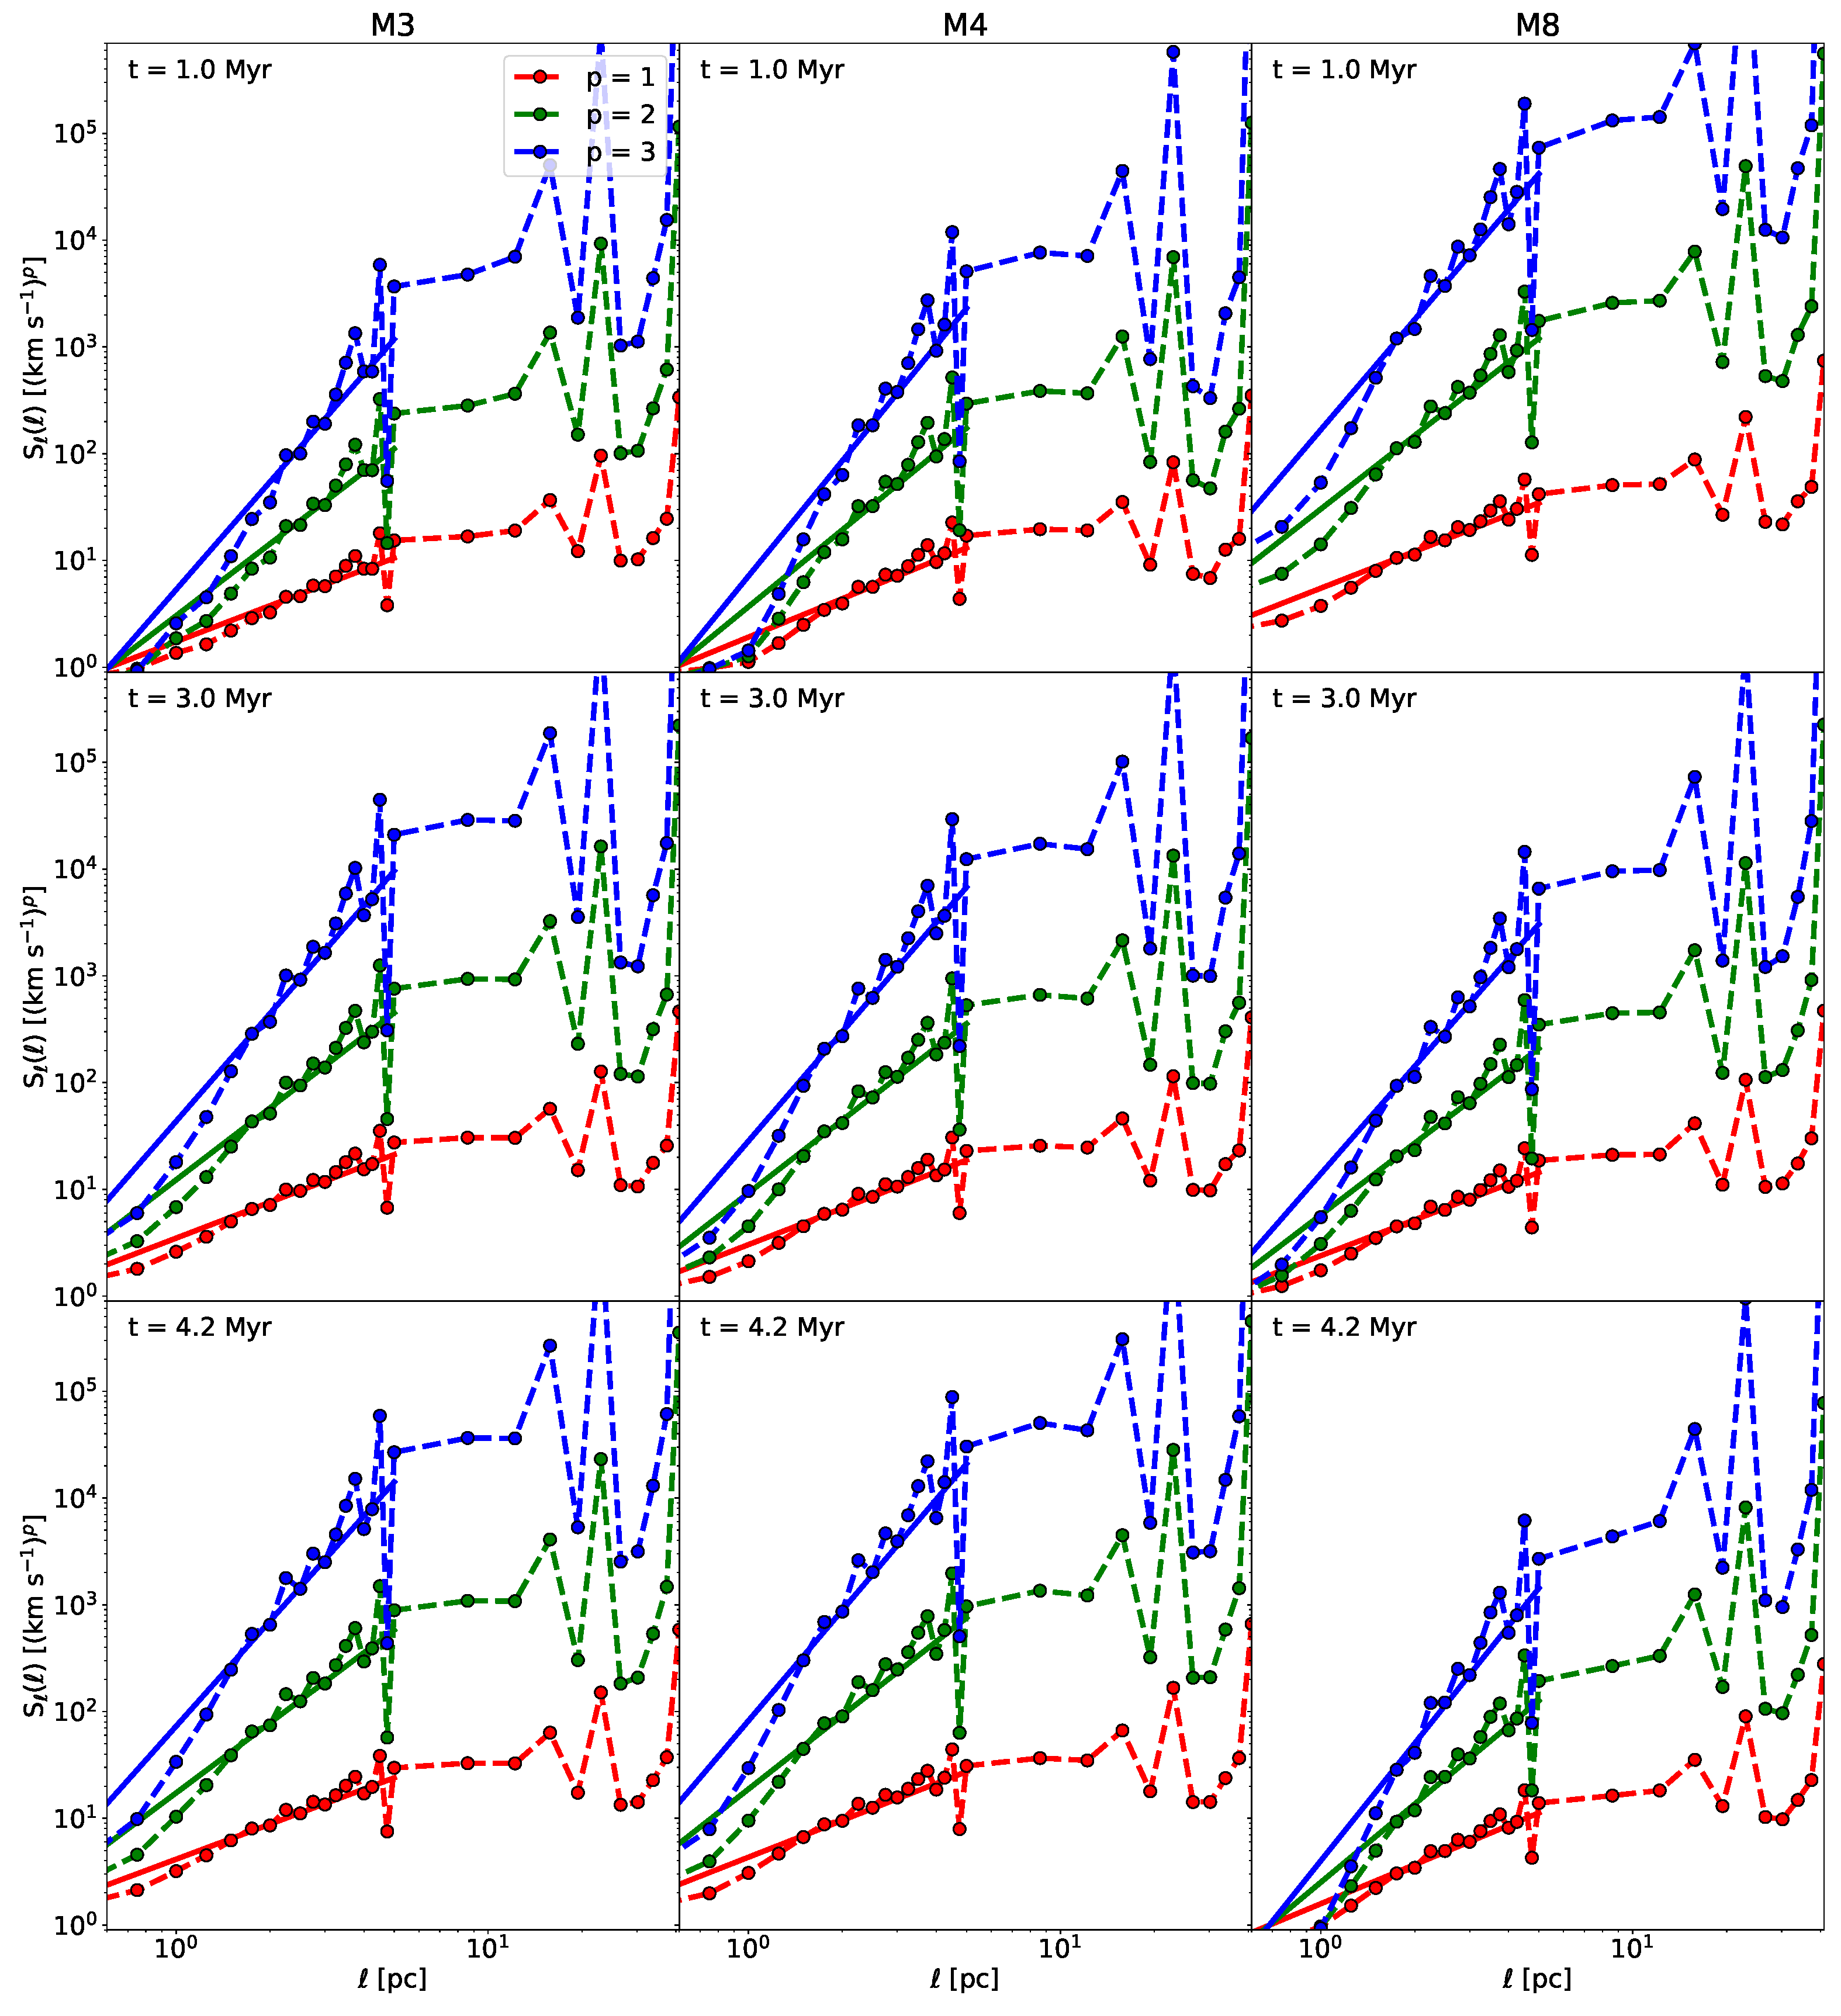
\includegraphics[width=\textwidth]{app_examples_woutthres_s_l.pdf}
    \caption{
        As Fig.~\ref{pic:appInertial:examples_with_threshold_s_vs_l}, but based on data without density threshold.
    }
    \label{pic:appInertial:examples_without_threshold_s_vs_l}
\end{figure*}
 	
 	
\begin{figure*}
    \centering
    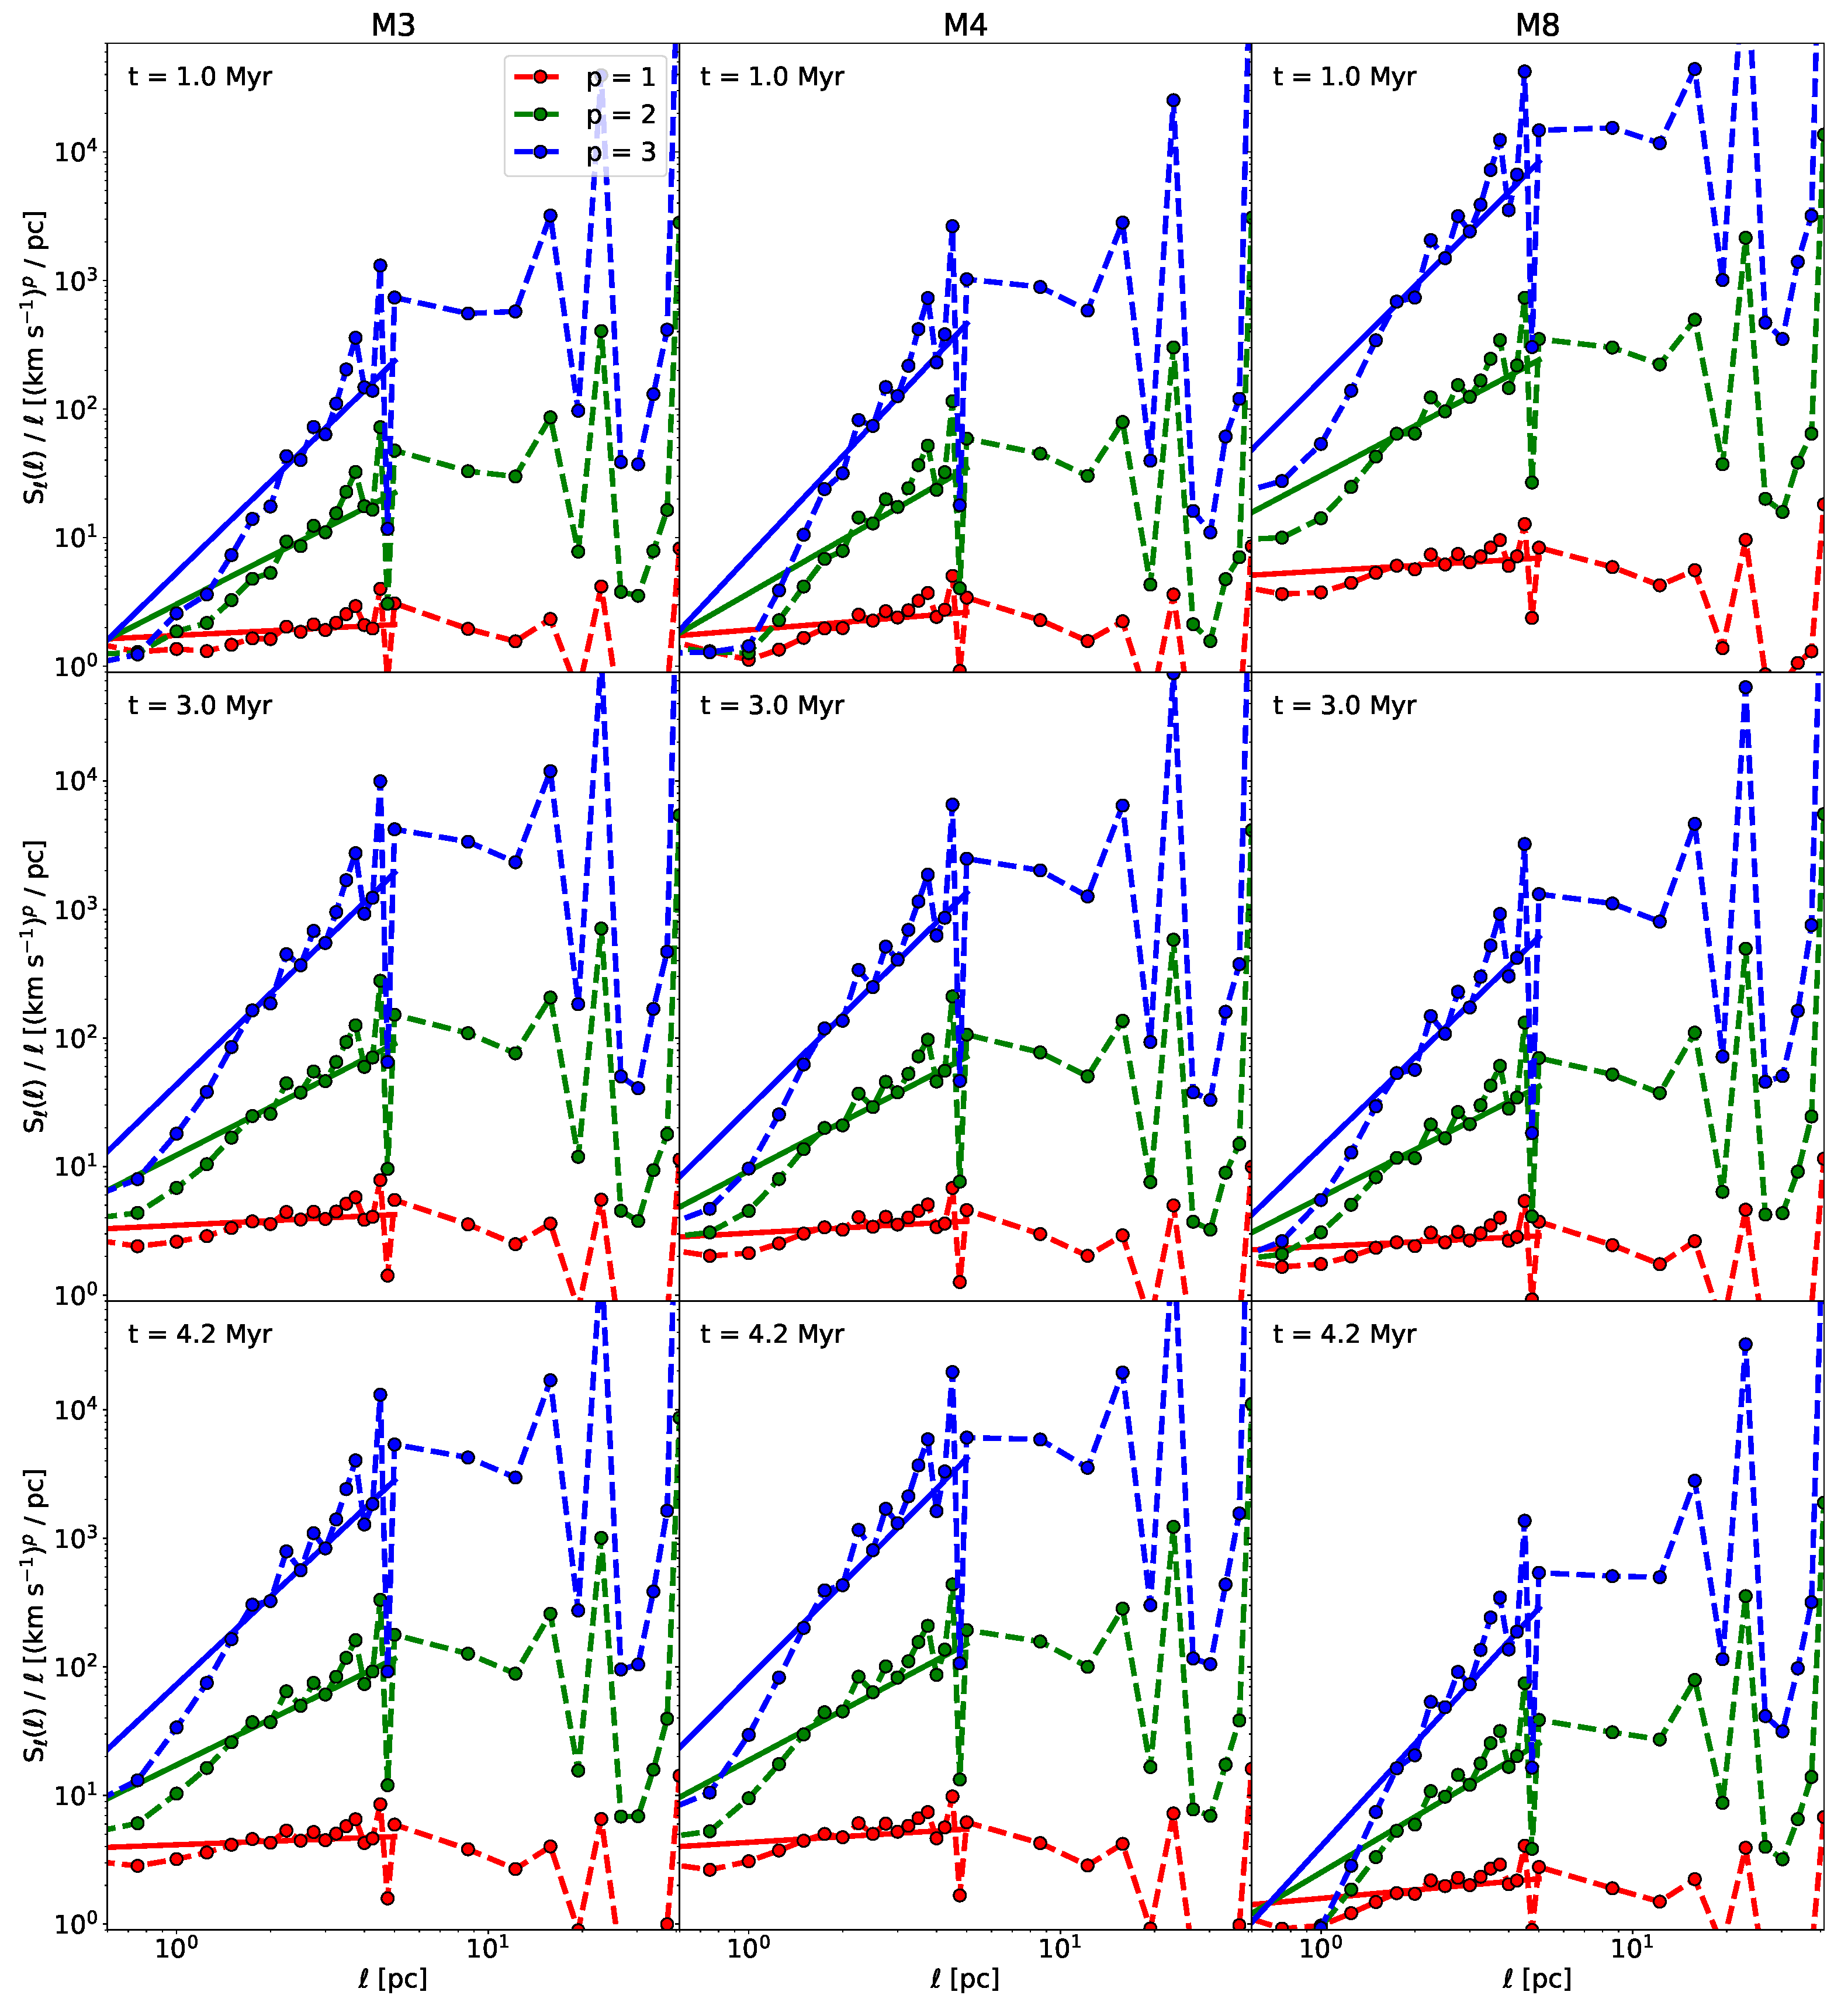
\includegraphics[width=\textwidth]{app_examples_woutthres_sl_l.pdf}
    \caption{
        As Fig.~\ref{pic:appInertial:examples_with_threshold_sl_vs_l}, but based on data without density threshold.
    }
    \label{pic:appInertial:examples_without_threshold_sl_vs_l}
\end{figure*}


 	
\begin{figure*}
    \centering
    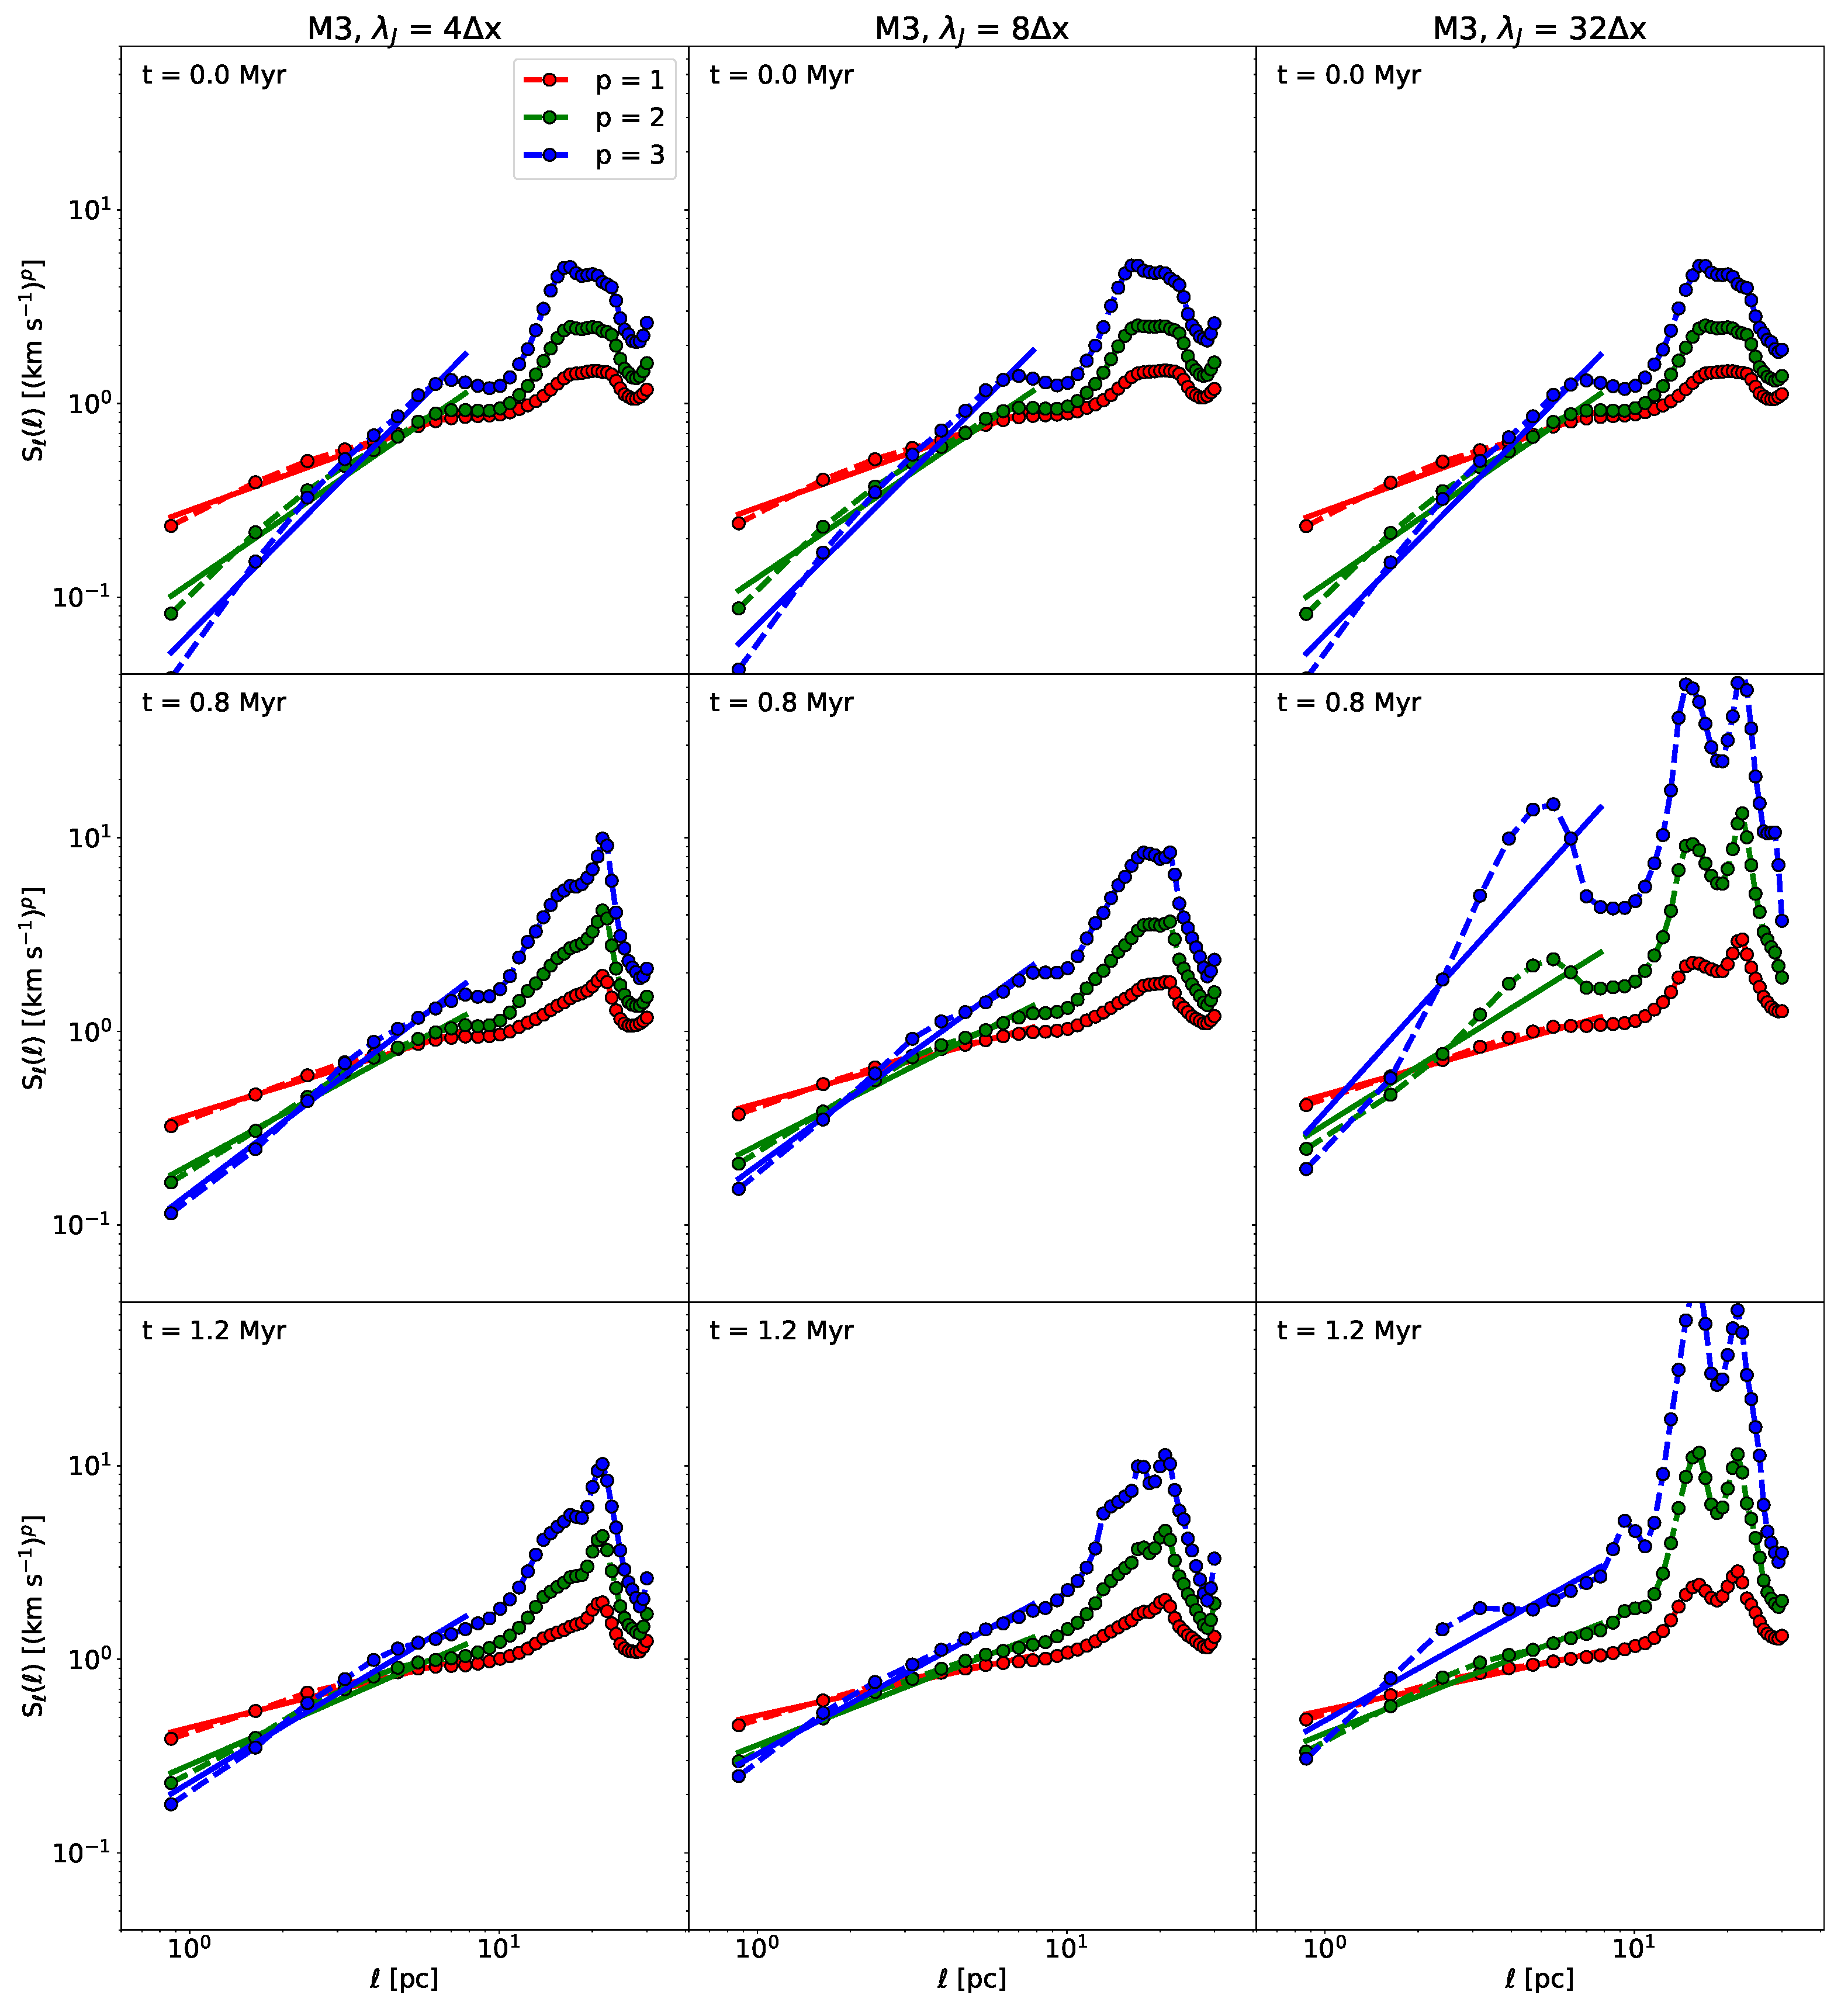
\includegraphics[width=\textwidth]{app_examples_jeans_s_l.pdf}
    \caption{
        The figures show additional examples of VSFs, based on data of \texttt{M3} with density threshold, at the different refinement levels (\textit{left} to \textit{right}) $\lambda$~=~4~$\Delta$x, $\lambda$~=~8~$\Delta$x, and $\lambda$~=~8~$\Delta$x as function of lag scale $\ell$ and order $p$. 
        The examples are given for three different time steps, namely (\textit{top} to \textit{bottom}) t~=~0.0~Myr, 0.8~Myr, and 1.2~Myr.
        The dots (connected by dashed lines) show the values computed from the simulations. 
        The solid lines represent the power-law relation fitted to the respective structure functions.
    }
    \label{pic:appInertial:examples_jeans_s_vs_l}
\end{figure*}


 	
\begin{figure*}
    \centering
    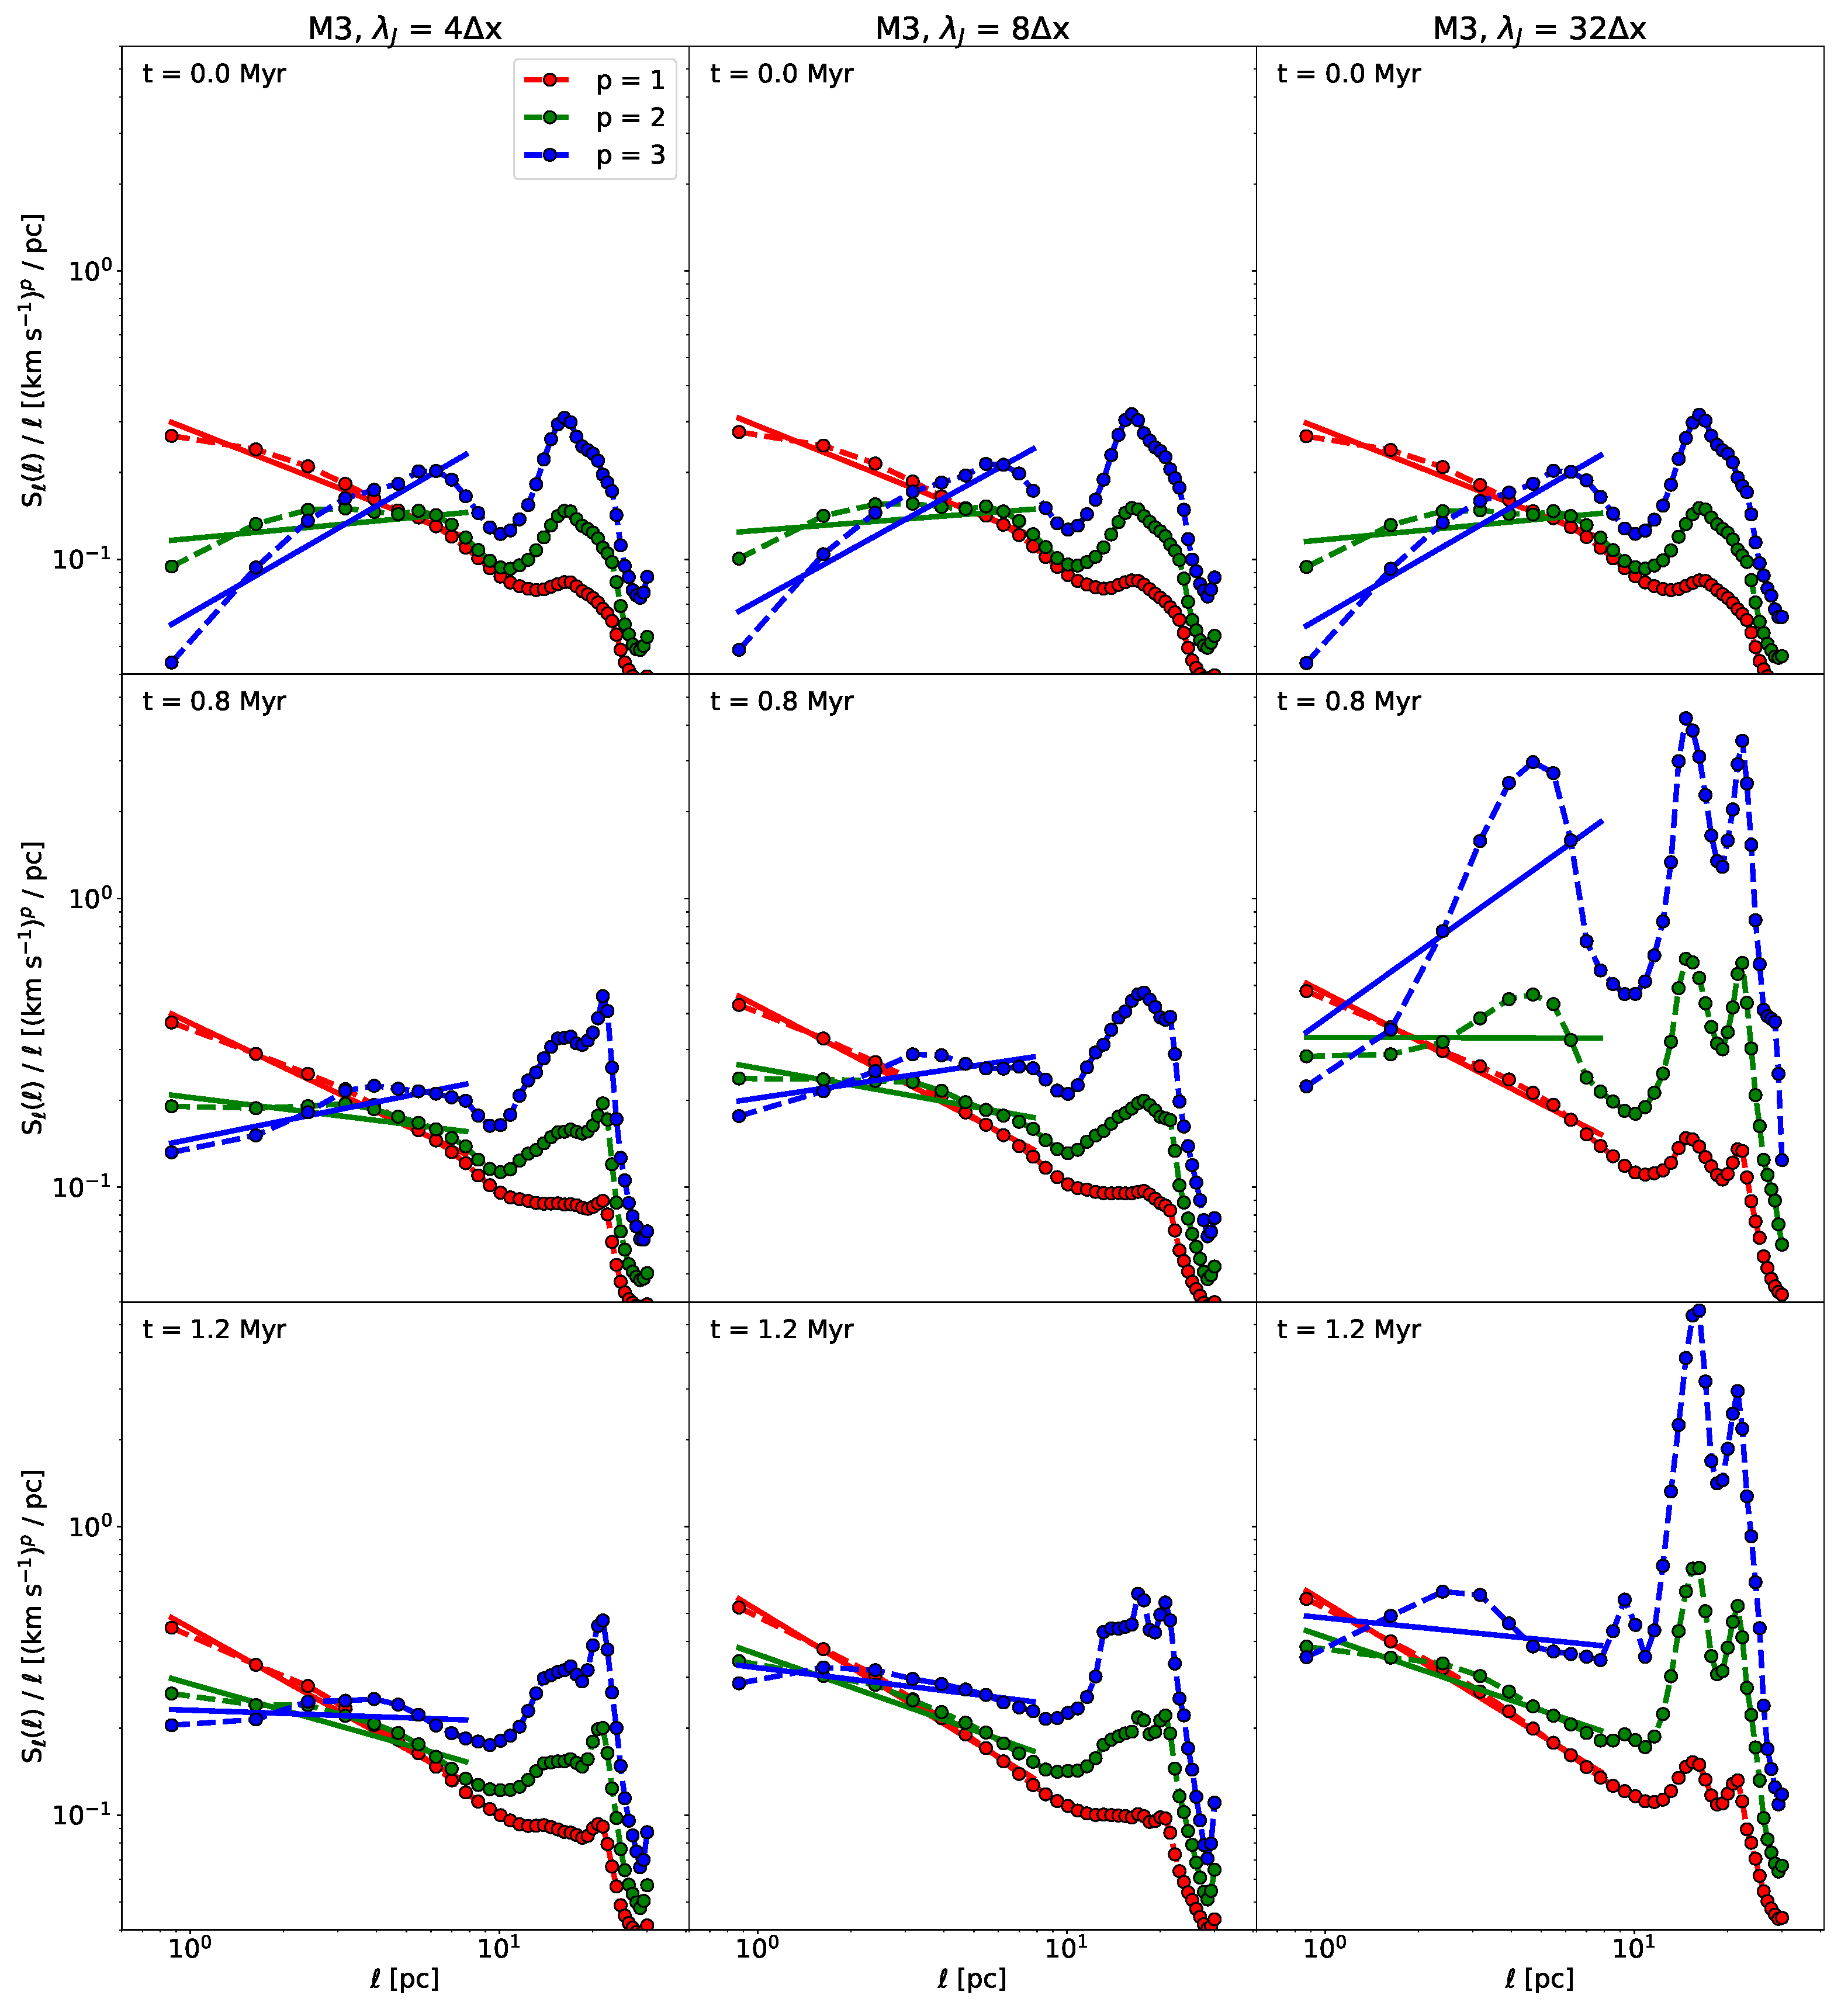
\includegraphics[width=\textwidth]{app_examples_jeans_sl_l.pdf}
    \caption{
        As Fig.~\ref{pic:appInertial:examples_jeans_s_vs_l}, but plotting the relation between S$_{\ell}$ / $\ell$ as function of lag scale $l$ and order $p$.
    }
    \label{pic:appInertial:examples_jeans_sl_vs_l}
\end{figure*}


\textbf{
    The figures are similar to the examples shown in Fig.~\ref{pic:results:vsf_example}, but with data from all three clouds and at three different snapshots during the simulations.
    The straight lines within the plots indicate the power-law relation that we have fitted onto the VSFs, considering the range $\ell\,\leq$~8~pc.
}

\textbf{
    We see that in most of the cases the VSFs are in good agreement with the described power-law relation within the fitted ranges (e.g., Fig.~\ref{pic:appInertial:examples_with_threshold_s_vs_l}). 
    Yet, there are cases when the VSF is not well reproduced by a simple, single power-law function.
    Examples are: \texttt{M3} at $t$~=~3.0~Myr in Fig.~\ref{pic:appInertial:examples_with_threshold_s_vs_l} or \texttt{M3} at $t$~=~0.8~Myr and with $\lambda_\mathrm{J}$~=~32$\Delta$x in Fig.~\ref{pic:appInertial:examples_jeans_s_vs_l}.
    In the first case, the dominating source of turbulence within the cloud is switching of large-scale driving to contraction-driven. 
    This means that the outer regions of the clouds (larger $\ell$) are still dominated by external driving, while the inner regions (smaller $\ell$) start accelerate mostly due to fragmentation and infall motions.
    The consequence is that the actual VSF is a super-position of two processes that amplify the relative motions of the gas portions differently and on different scales.
    A single power-law is incapable to reproduce this scenario adequately. 
    However, this occurs only in a few time steps of all the simulations. 
}

\textbf{
    The second example represents a VSF of a cloud that is interacting with a SN blast wave.
    In this case the maximal amplification is neither on the far end of the cloud, where the turbulence is driven by external sources, nor on small scales where gravitational contraction acts.
    Instead the (local) maximum is the intermediate scale. 
    Considering the morphology of the cloud and the cloud's environment this can only occur when the shock front of a SN is currently propagating through the cloud. 
    Thus, the VSF here is a super-position of three driving mechanisms: first, the external large-scale driving; second, self-gravity that leads to contractive motions; and the shock jump that injects large amounts of kinetic energy as it moves through the cloud. 
    The effect of latter, however, is only locally and short-living as the injected turbulence decays quickly (compare with \texttt{M3} at $t$~=~1.2~Myr and with $\lambda_\mathrm{J}$~=~32$\Delta$x in Fig.~\ref{pic:appInertial:examples_jeans_s_vs_l}).
}

\textbf{
	Note that we have also problems to describe the behaviour of small-scale motions (with $\ell\,\lesssim$~2~pc) when examining the data without applying a density threshold (see Figs.~\ref{pic:appInertial:examples_without_threshold_s_vs_l} and~\ref{pic:appInertial:examples_without_threshold_sl_vs_l}).
	In this case we study the turbulent motions within the ISM. 
	Contrary to the modelled molecular clouds, the ISM is not organised in hierarchical structures.
	Consequently, there are less differences in relative velocity between two cells that are close to each other, as the ISM is relatively homogeneous. 
	Within the clouds there are large gradients of relative velocities as two gas cells behave completely differently to each other depending on whether the connection line is parallel or perpendicular to one of the filaments.
	Furthermore, the turbulence within the ISM is dominantly driven by SN explosions only.
	This is why the gas motions here are more chaotic and irregular than within the clouds where the flows are regulated and united by the hierarchical structures and self-gravity.
	Yet, we see that our can fit the VSFs within the intermediate lag scale ranges (2~pc~$\lesssim\,\ell\,\lesssim$~8~pc). 
	Within this range the models can moderately well reproduce the inertial range of the turbulent cascade, making it a good basis for the analysis we have presented in the main part of this paper.
}











